\part{Implementación}\label{part:implementacion}

\section{Hardware}

\section{Programa del microcontrolador} \label{sec:sw-implementacion}

\subsubsection{Plataformas de desarrollo}\label{sec:sdk}
El System on Chip ESP8266EX es muy popular y existen diversas formas de desarrollar para él, entre ellas están:
\begin{itemize}
	\item El SDK oficial \enquote{OS} de Espressif. Es un SDK privativo. Utiliza internamente FreeRTOS con lo que se puede programar con tareas y las primitivas de sincronización que FreeRTOS ofrece.
	\item El SDK oficial \enquote{NON-OS} de Espressif. Tiene \enquote{NON-OS} en su nombre porque con este SDK el programador no puede especificar ni crear tareas propias. Sino que se limita a registrar funciones callbacks que son llamadas por el firmware de Espressif cuando suceden eventos. La programación termina siendo basada en eventos.
	\item La implementación de la plataforma Arduino para el ESP8266EX. Es la más sencilla de utilizar. Tiene las mismas abstracciones que se utilizan en la plataforma Arduino original. Incluye clases C++ que implementan servidores HTTP y hay mucho software y soporte disponible.
\end{itemize}

Todas estas formas de desarrollar tienen en común que el software del programador corre sobre un firmware privativo, es decir, no es viable programarlo \enquote{bare-metal} porque los registros y todos la información del hardware necesario para realizar algo no trivial no está disponible.

Para el este proyecto se decidió utilizar el SDK \enquote{NON-OS}, donde las funciones que define el programador se ejecutan siempre enteramente, de forma cooperativa. Esto elimina toda una clase de problemas de interferencia de datos a causa de la concurrencia, con lo que no es necesario utilizar primitivas de sincronización.

Un ejemplo de esta técnica de programación se puede ver en la figura \ref{fig:callbacks}, donde se muestra como se registra la función que debe ejecutarse al recibir datos a través de una conexión TCP sobre 802.11. La aplicación llama a \code{espconn\_regist\_recvcb}, pasándole un puntero a función a \code{callback} y el firmware se encarga de llamar a \code{callback} cuando corresponda.

\begin{figure}[ht!]
	\begin{center}
		\centering
		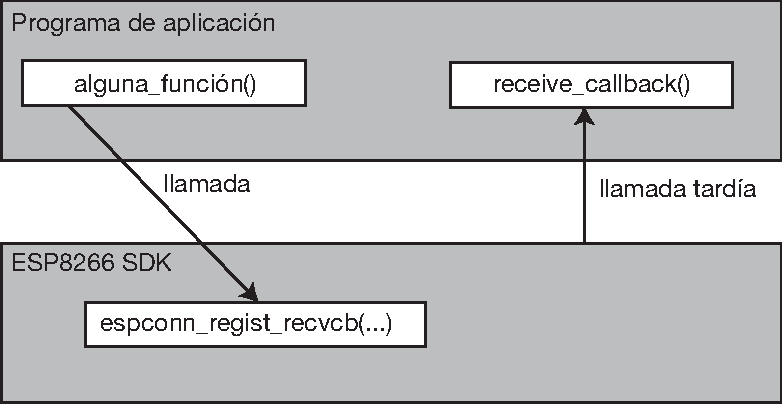
\includegraphics[scale=0.8]{imagenes/callbacks.pdf}
		\caption{Ejemplo de uso de callbacks.}
		\label{fig:callbacks}
	\end{center}
\end{figure}

\subsubsection{Archivo principal} \label{sec:archivo_principal}

\lstinputlisting[label=pseudo:userInit, linerange=1-10, firstnumber=1] {codigo/pseudocodigo/microcontrolador.pseudo}

El Archivo principal del programa que corre sobre el microcontrolador es el archivo main.cpp.
Dentro tiene un método denominado \code{user\_init()} que actúa como punto de entrada de la aplicación y no contiene parámetros.
En su definición se inicializa cada clase mencionada en la sección previa, ejecutando el método init( ) de cada una de ellas.
Dicho método es el encargado de asignar los valores iniciales a las variables internas de cada módulo de software, de forma de poder usar sus servicios públicos, posteriormente.
Éstas clases son las que se observan en la figura \ref{fig:flujo_de_datos}: WiFiManager, LedSign, Server y Settings.

Adicionalmente se establece tasa de bits por segundo a 115200 por medio de una función propia del SDK utilizado para el desarrollo.
Por último para utilizar los pines del micro, se inicializan los GPIO del microcontrolador, a través de la función gpio\_init( ) que también es propia del SDK.
En el fragmento \ref{pseudo:userInit} se muestra un pseudocódigo del método user\_init\( \).

Por último, se observa que para la clase Settings, se ejecuta el método loadSettings( ).
El mismo se encarga de cargar desde la memoria no volátil del microcontrolador, la última información almacenada respecto del texto a mostrar en el cartel, sus parámetros de configuración, y sus valores de red. \newline

\subsubsection{Settings}

La clase Settings es la encargada de mantener en memoria RAM, la información principal respecto del cartel.
Entre ellas, contiene el texto a mostrar, su velocidad de parpadeo y desplazamiento y la información de la red a la que actualmente se encuentra conectado el sistema.
Además posee funcionalidades para almacenar dichos datos en memoria no volátil a fin de persistirlos ante un reinicio.
En la figura \ref{uml:settings}, se observa un diagrama UML con los principales métodos de la clase en cuestión, y a continuación se describe cada uno de ellos.

\begin{figure}[!ht]
	\centering
	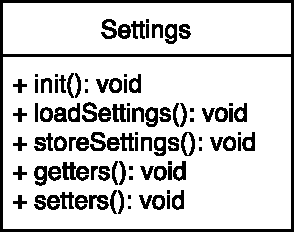
\includegraphics[scale=0.8]{imagenes/uml/settings.pdf}
	\caption{UML de la clase Settings.}
	\label{uml:settings}
\end{figure}

\lstinputlisting[linerange=12-12, firstnumber=12] {codigo/pseudocodigo/microcontrolador.pseudo}

El método \code{init()} de settings se encarga de inicializar el puntero de la estructura de la flash de donde lee y almacena los datos.
Adicionalmente, la clase provee funcionalidad para establecer las configuraciones por defecto del sistema, presionando el botón de RST durante 5 segundos.
Para lograr eso, dentro del método \code{init()} también se inicializa el pin que se va a utilizar como reset (pin GPIO2) y se establece el callback para cuando dicho evento ocurra.
Se recomienda revisar la sección \ref{sec:sdk} donde se explica el mecanismo de callbacks que utiliza el microcontrolador.

\lstinputlisting[linerange=14-14, firstnumber=14] {codigo/pseudocodigo/microcontrolador.pseudo}

El método \code{loadSettings()} se encarga de cargar en memoria RAM la información necesaria del cartel utilizando el puntero previamente incializado en \code{init()}.
Adicionalmente se le envía, dicha información, a la clase LedSign quien es la encargada de mostrar el contenido anteriormente almacenado en la memoria.

En caso de que la información leída estuviese corrupta, la clase contiene un método privado para cargar los datos por defecto del sistema.
El método no posee parámetros.

\lstinputlisting[linerange=16-16, firstnumber=16] {codigo/pseudocodigo/microcontrolador.pseudo}

El método \code{storeSettings()} de la clase Settings provee funcionalidad para almacenar en la memoria no volátil la información actual del sistema.
Para la persistencia de los datos, se utiliza la librería propietaria del SDK denominada spi\_flash.h.
Este método no contiene parámetros.


\subsubsection{WiFiManager}

La clase WiFiManager es la encargada de administrar todas las configuraciones WiFi que necesita el microcontrolador para conectarse a una red.
Posee un sólo método público enunciado en el apartado \ref{sec:archivo_principal}, denominado init( ).

\lstinputlisting[linerange=18-18, firstnumber=18] {codigo/pseudocodigo/microcontrolador.pseudo}

El método no contiene parámetros y su principal tarea consiste en leer los datos de la clase Settings relacionados a la información de la red.
Dichos valores corresponden al SSID, contraseña de WiFi, ip, y máscara de subred y son utilizados para permitir al sistema conectarse a la red WiFi correspondiente.
La librería propia del SDK osapi.h permite realizar estas acciones.



\subsubsection{Server}

Una vez conectado a la red WiFi, la clase Server es la encargada de colocar al microcontrolador en modo servidor, de forma de poder atender las peticiones que realiza el usuario.
Provee funcionalidades para inicializar el servidor, desconectar la sesión, enviar mensajes hacia el cliente, y notificar cuando se recibe un paquete.
En el UML de la figura \ref{uml:server} se observan los métodos públicos de la clase que abstrae las funcionalidades mencionadas anteriormente.

\begin{figure}[!ht]
	\centering
	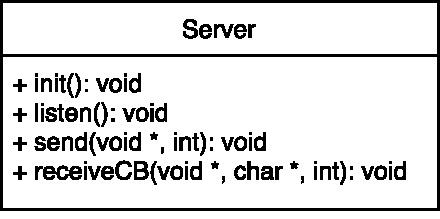
\includegraphics[scale=0.8]{imagenes/uml/server.pdf}
	\caption{UML de la clase Server.}
	\label{uml:server}
\end{figure}

Cabe destacar que en la figura \ref{uml:server} aparece una función privada relacionada a la recepción de mensajes denominada \code{receiveCallback()}.
Como bien su nombre lo indica, esto es un callback que se setea dentro del método \code{listen()} y se ejecuta cuando algún paquete llega al servidor (para más información, revisar la sección \ref{sec:sdk} donde se explica el método de callbacks).
A pesar de que sea un método privado, se decide mostrar en el UML debido a su reelevancia en esta solución.
Más adelanete, en esta sección, se explica su implementación.

\lstinputlisting[linerange=20-20, firstnumber=20] {codigo/pseudocodigo/microcontrolador.pseudo}

El método \code{init()} de la clase Server se ejecuta en el archivo principal y su función esencial consiste en inicializar las variables internas de la estructura de modo de permitir, posteriormente, colocar al microcontrolador en modo servidor.
Cabe aclarar que esta función debe ejecutarse después de haberse autenticado a una red WiFi; por ese motivo, primero se ejecta el \code{init()} de la clase WiFiManager.
Por otra parte, éste método no coloca al programa en modo servidor, es decir, no permite que distintos clientes se conecten todavía; para ello debe ejecutarse el método \code{listen()} que se describe a continuación.

\lstinputlisting[linerange=22-22, firstnumber=22] {codigo/pseudocodigo/microcontrolador.pseudo}

En primer lugar, el método \code{listen()} configura el certificado y la clave de seguridad del protocolo SSL que se utiliza en el intercambio de mensajes entre el servidor y el cliente de forma de que los mismos permanezcan cifrados hasta llegar a destino.
Adicionalmente, activa el mecanismo de Keep Alive propio de TCP, limita el número de conexiones simultáneas a uno y registrar los callbacks necesarios para su correcto funcionamiento (entre ellos el correspondiente a la recepción de paquetes).
El método no contiene parámetros.

\lstinputlisting[linerange=24-24, firstnumber=24] {codigo/pseudocodigo/microcontrolador.pseudo}

El método \code{send()} provee funcionalidad para enviar mediante TCP, hacia el cliente, un arreglo de bytes de manera cifrada.
Para su utilización, es necesario haber ejecutado el método \code{listen()} previamente y haber establecido una conexión con un cliente.

Recibe como parámetro un puntero que contiene la dirección del mensaje a enviar y el tamaño de dicho paquete.

\lstinputlisting[label=pseudo:receiveCallback, linerange=26-32, firstnumber=26] {codigo/pseudocodigo/microcontrolador.pseudo}

Como ya se mencionó anteriormente, el método \code{receiveCallback()} es una función privada que se ejecuta sólo cuando se reciben datos desde el cliente (size).
Contiene un buffer interno donde almacena los bytes que obtiene.
Los parámetros que recibe corresponden con la conexión vía TCP que envía los datos (conn), un puntero a la cadena de bytes recibido (data) y por último el tamaño de dicho arreglo.

Dicha estructura posee una capacidad limitada y, en este caso, su tamaño máximo se especifica en el protocolo de software (ver sección \ref{sec:protocolo}).
Cabe aclarar que la tarea de este método es acumular bytes hasta llenar el buffer. La clase Server no tiene las herramientas necesarias para interpretar la información que recibe.
Por ese motivo cuando la estructura se llena, se notifica a la clase MessageHandler quien es la que implementa el protocolo de comunicación diseñado para este proyecto y es quien es capaz de interpretar la secuencia de bytes recibida.



\subsubsection{MessageHandler}

La clase MessageHandler implementa el protocolo de comunicación entre el servidor y el cliente, y es capaz de interpretar el arreglo de bytes que recibe desde la clase Server.
Esta clase contiene un sólo método denominado \code{handle()} que atiende el mensaje que le envía el usuario y genera una respuesta para el cliente.
En el fragmento \ref{pseudo:messageHandlerHandle} se muestra un pseudocódigo del método a fin de brindar mayor claridad en la comprensión de la función.

\lstinputlisting[label=pseudo:messageHandlerHandle,linerange=36-93, firstnumber=36] {codigo/pseudocodigo/microcontrolador.pseudo}



\subsubsection{LedSign}

La última clase de la arquitectura del programa del microcontrolador es LedSign.
La misma se encarga de recibir los datos que envía MessageHandler por parámetro, procesarlos y armar un buffer de salida con la información necesaria para encender las luces de la matriz.
Cabe recordar que el programa del microcontrolador solo se comunica con el primer MAX7219 como lo indica la figura \ref{fig:flujo_de_datos}.
En la figura \ref{uml:ledSign} se muestra un UML con los métodos públicos que componen la clase.

\begin{figure}[!ht]
	\centering
	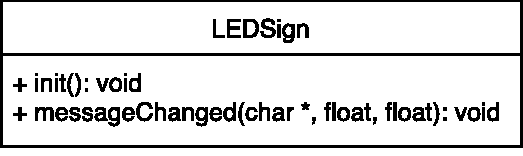
\includegraphics[scale=0.8]{imagenes/uml/LEDSign.pdf}
	\caption{UML de la clase LEDSign.}
	\label{uml:ledSign}
\end{figure}

\lstinputlisting[linerange=95-109, firstnumber=95] {codigo/pseudocodigo/microcontrolador.pseudo}

En primer lugar, el método \code{init()} se encarga de configurar los pines LATCH, CLK y DATA que se utilizan para la comunicación entre el microcontrolador y el MAX7219.
Para mayor información respecto de los pines, se sugiere visitar la sección \ref{sec:hw} %TODO AMG - poner la sección donde se explica los pines esos.

Adicionalmente se configura como salida los pines que se utilizan para los jumpers, se les habilita su pull up interno y se lee su valor a la salida.
De esta forma, se indica cuántos módulos de 8x8 LEDs componen el cartel.

Por otra parte, el método se encarga de configurar todos los registros necesarios de cada MAX7219 para iniciar su funcionamiento.
Entre las acciones que realiza, el programa se encarga de sacarlo del modo test, configurar la intensidad de los LEDs, indicarle que se van a usar las ocho columnas que posee el chip, limpiarle la pantalla apagando todos los LEDs y encenderlo.
Dichas configuraciones se realizan través del método \code{sendCommand()}.
La función toma dos parámetros, en el primero se especifica el registro a configurar y en el segundo el valor que se desea establecer.
Para más información respecto de la configuración de los registros consultar el datasheet del MAX7219 haciendo click en el siguiente \href{https://datasheets.maximintegrated.com/en/ds/MAX7219-MAX7221.pdf}{link}.

Finalmente se limpia el cartel, apagando todas las luces de cada módulo.

\lstinputlisting[linerange=111-111, firstnumber=111] {codigo/pseudocodigo/microcontrolador.pseudo}

El método \code{messageChanged()} se invoca cuando el mensaje o algún parámetro de configuración (tiempo de parpadeo o velocidad de desplazamiento) es modificado.

Recibe tres parámetros de configuración, el primero es el texto a mostrar.
Éste es un puntero a char donde se encuentra la información del contenido.
Es necesario que tenga un terminador nulo.
En caso de que no lo tenga, el comportamiento del método queda indefinido.

El segundo parámetro es brate, es un float que indica la velocidad de parpadeo que posee el texto.
Un valor negativo, repercute en comportamiento indefinido.
En caso de que no se requiera se debe colocar un 0.

El último parámetro es srate que también es un float que indica la velocidad a la que se desplaza el contenido.
La diferencia con el anterior radica en que este sí puede tomar valores negativos.
Un valor negativo indica que el contenido se desplaza a la izquierda, mientras que un positivo lo hace hacia la derecha.
En caso de que no se requiera el uso de esta funcionalidad, se debe colocar un 0. 

La función principal de este método es tomar los datos de configuración que se reciben por parámetro y armar un buffer de salida con la información de cada columna del cartel, respecto del estado de cada LED.
Para realizar el desplazamineto del contenido, la estrategia que se adopta es periódicamente, mover el índice del buffer y enviar nuevamente la información al MAX7219.
Para el tiempo se utiliza una estructura propia del SDK del microcontrolador denominado timer\_t.
La misma permite ejecutar un callback cuando se cumple un determinado lapso de tiempo.

Para realizar el parpadeo del mensaje, se adopta una estrategia similar.
Basándose en otro timer\_t se envía periódicamente un comando a cada MAX7219 que le indica que debe encenderse o apagarse, según corresponda.

\section{Aplicación de PC}\label{sec:pc}
La aplicación de PC es un programa con interfaz gráfica que permite al usuario administrar el contenido y configuración del cartel de forma remota. En el marco del protocolo definido en el \ref{sec:protocolo}, la aplicación de PC es el cliente.

\subsubsection{Plataforma de desarrollo}
La aplicación está desarrollada en el \emph{framework} de desarrollo Qt. Qt es un conjunto muy amplio de librerías que permiten el desarrollo de aplicaciones gráficas que se pueden compilar para distintas plataformas (Windows, GNU/Linux, macOS o cualquier variante de Unix con X11). El lenguaje de programación que se utiliza es C++ con extensiones propias de Qt.

\subsubsection{Arquitectura basada en eventos}\label{sec:qt}
Qt permite desarrollar aplicaciones con una arquitectura basada en eventos. Sin embargo, la implementación de este sistema de eventos no está basada en los mecanismos más clásicos como el patrón Observer de la programación orientada a objetos ni el mecanismo de callbacks o punteros a funciones propios de la programación procedural, sino que hay métodos en los objetos que pueden ser denominados \emph{signals} o \emph{slots}.

Una clase puede tener opcionalmente uno o más métodos que sean \emph{signal} o \emph{slot}. La idea clave de estas sistema es que un objeto puede \enquote{emitir} una \emph{signal} que ejecuta el método \emph{slot} de otro objeto (o incluso posiblemente el mismo emisor) al cual se estableció previamente lo que se denomina \enquote{conexión}. Se ilustra este mecanismo en la figura \ref{fig:signals-slots}

\begin{figure}[!ht]
	\centering
	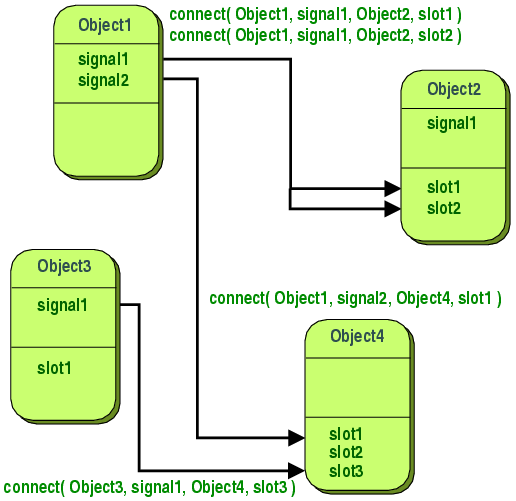
\includegraphics[height=8cm]{imagenes/signal-slots.png}
	\caption{Mecanismo de \emph{signal} y \emph{slot}.}
	\label{fig:signals-slots}
\end{figure}

En Qt, las clases que necesiten utilizar el sistema de eventos deben heredar de una clase provista por la librería llamada \code{QObject}. Esta clase provee distintas funcionalidades al resto de las clases definidas por Qt. Entre los objetos que heredan de QObject puede existir una relación de parentesco, en la cual un objeto $B$ puede tener como padre a otro objeto $A$. Esto, por ejemplo, sirve para liberar al programador del manejo de memoria: un objeto puede destruir a sus hijos antes de destruirse a sí mismo (por destrucción se entiende la liberación de todo recurso asociado al objeto, como memoria o archivos).

El mecanismo de \emph{signal} y \emph{slots} tiene como una de sus ventajas el hecho de que la ejecución de un \emph{slot} darse en otro hilo. Esto esta relacionado con la idea que promueve Qt de que un objeto puede \enquote{pertenecer} a un hilo de ejecución (encapsulado por la clase \code{QThread}), esto permite que no haya interferencia de datos causada por la concurrencia ya que no hay accesos explícitos a variables compartidas entre hilos sino que pueden enviar datos como argumentos a los \emph{slots}, de forma similar al paradigma de pasaje de mensajes en programación concurrentes.

Por ejemplo, en el caso del objeto \code{Object1} en la figura \ref{fig:signals-slots}, en algún método suyo se podría tener código como el siguiente:
\begin{lstlisting}[language=c++]
	// ...
	emit signal1();
	// ...
\end{lstlisting}

Mientras que \code{Object2} tiene un \emph{slot} llamado \code{slot1()} al cual \code{signal1()} de \code{Object1} está conectado. Entonces al emitirse \code{signal1()}, se ejecuta también \code{slot1} de \code{Object2} (además de los otros métodos pertenecientes a las otras clases que aparecen en la figura).

El momento en que se ejecuta un \emph{slot} depende del tipo de conexión que se haya establecido entre los objetos. Qt define tres tipos de conexiones:
\begin{description}
	\item[\code{DirectConnection}:] el \emph{slot} se ejecuta en el mismo hilo de ejecución desde el cual se hizo la emisión. Esto es útil para cuando los objetos que están conectados pertenecen a un mismo hilo o también cuando pertenecen a distintos hilos pero se toma precaución utilizando primitivas de sincronización para serializar el acceso al recurso o memoria compartida.
	\item[\code{QueuedConnection}:] se coloca un pedido de ejecución de \emph{slot} (con los argumentos que se hayan emitido) en la cola de eventos del hilo del objeto destino. Esto es lo que libera al programador de tener que utilizar primitivas de sincronización explícitas y es lo que se usa mayormente en la aplicación de PC de este proyecto. La ejecución de \code{emit} retorna inmediatamente, con lo que el hilo del objeto emisor no se bloquea al emitir una señal.
	\item[\code{BlockingQueuedConnection}:] Similar a \code{QueuedConnection}, con la diferencia que el hilo emisor se bloquea hasta que finalice la ejecución de los \emph{slots} que haya activado. Si no se utiliza con precaución y se establecen conexiones cíclicas, existe el riesgo de que ocurra un \emph{deadlock}, ocurrencia en la que un conjunto de hilos se espera entre sí indefinidamente, deteniendo parcial o íntegramente el programa.
\end{description}

Internamente, la implementación de Qt tiene una cola bloqueante de eventos para cada uno de los hilos que tengan una instancia de la clase \code{QThread}. También lleva registro de cuáles objetos que heredan de \code{QObject} pertenecen a cuál hilo. De esta manera, la ejecución de un hilo consiste principalmente en esperar a que hayan eventos para procesar en una cola bloqueante, cuya implementación específica depende de la plataforma para la cual se esté compilando el programa.

\subsubsection{Módulos}
En esta sección se listan las clases más relevantes de la aplicación de PC, sus métodos públicos principales y la interacción entre ellos.
Las clases son:
\begin{description}
	\item[\code{Panel}:] Provee la interfaz gráfica principal, que consiste en una ventana con los distintos elementos de control para que el usuario pueda manipular el cartel. Se puede ver una captura de pantalla en la figura \ref{fig:panel-screenshot}.
	\item[\code{Client}:] Realiza la interacción con el cartel a nivel mensaje del protocolo. Se encarga de generar los mensajes salientes y de tomar las acciones pertinentes ante una respuesta del cartel (servidor). La (única) instancia de esta clase \enquote{pertenece} (ver sección \ref{sec:qt}) a otro hilo en el cual se realizan todas las operaciones bloqueantes de entrada y salida, de forma que no se bloquea el hilo principal, que causaría que la interfaz gráfica deje de responder a eventos del sistema o del usuario.
	\item[\code{Connection}:] Abstrae la conexión al cartel, exponiendo métodos que envían y reciben específicamente los mensajes definidos en el protocolo. En esta clase también se hace la carga del certificado TLS antes de establecer una conexión.
	\item[\code{SignModel}:] Una clase \enquote{tonta} que agrupa todos los parámetros modificables del cartel, como el texto del cartel y sus parámetros de animación, los datos de la red Wifi a la que se debe conectar el cartel, etc. Existe principalmente para llevar registro de cuales parámetros fueron cambiados por el usuario y ameritan un pedido de cambio hacia el cartel. De manera que no se hagan cambios innecesarios al contenido o configuración del cartel.
\end{description}

Se puede ver en la figura \ref{fig:uml-cliente} un diagrama de los objetos mencionados anteriormente. No están incluidas las conexiones entre los objetos para mantener la prolijidad del diagrama.

Los objetos están repartidos entre los dos hilos como se muestra en la figura \ref{fig:qt-threads}.

\begin{figure}[!ht]
	\centering
	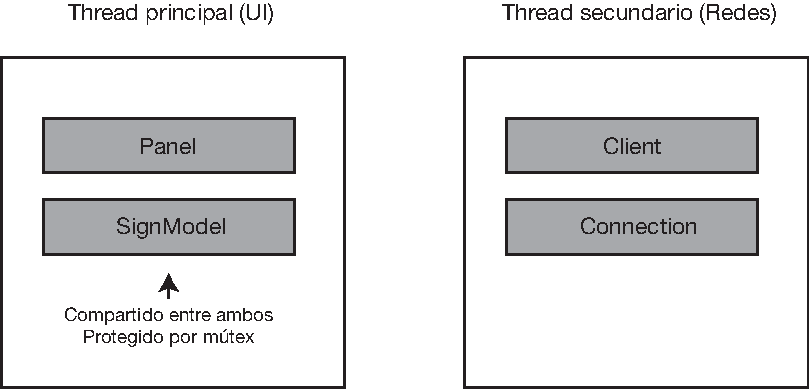
\includegraphics[scale=0.8]{imagenes/qt-threads.pdf}
	\caption{Distribución de los objetos en hilos.}
	\label{fig:qt-threads}
\end{figure}

\begin{figure}[!ht]
	\centering
	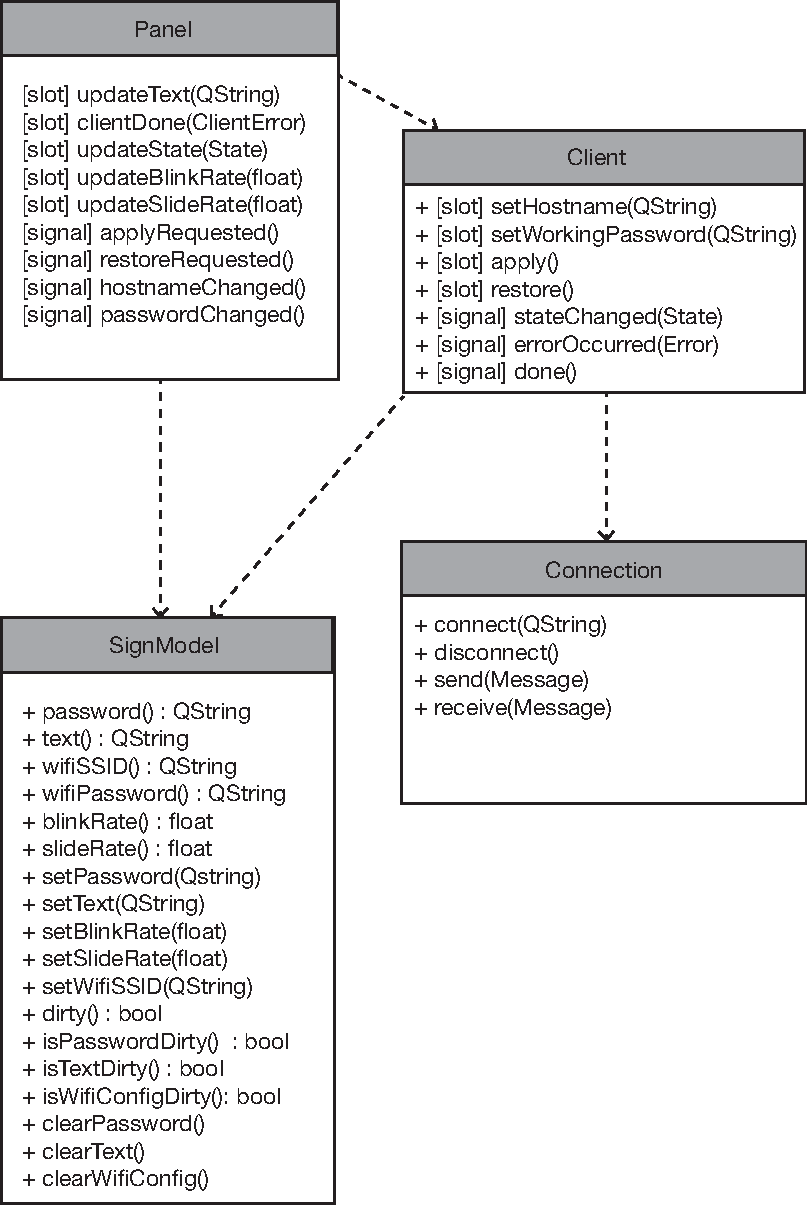
\includegraphics[scale=0.8]{imagenes/uml-cliente.pdf}
	\caption{Diagrama UML de las clases más relevantes.}
	\label{fig:uml-cliente}
\end{figure}

\begin{figure}[!ht]
	\centering
	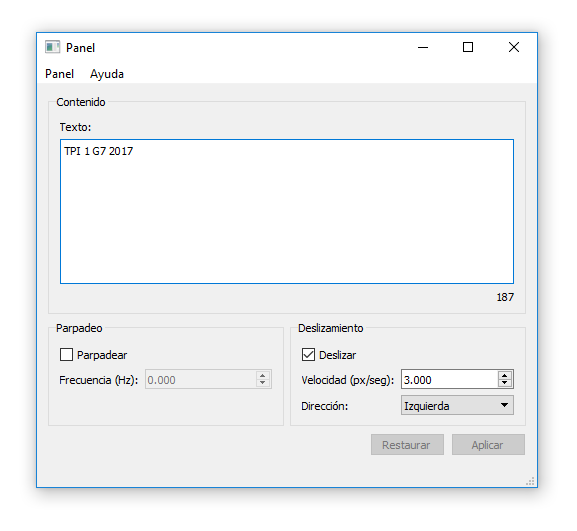
\includegraphics[height=10cm]{imagenes/panel-screenshot.png}
	\caption{Captura de pantalla de la ventana principal de la aplicación de pc.}
	\label{fig:panel-screenshot}
\end{figure}

\paragraph{Panel}
La clase Panel implementa la interfaz gráfica mediante la cual el usuario ingresa y visualiza el contenido y configuración del cartel. Sus métodos no deben hacer operaciones que tarden, ya que eso resultaría en que la interfaz de usuario se congele. Por esto y para lograr una mejor separación de propósito en las clases, la clase Panel solo se encarga de este aspecto del programa.

Un flujo típico de ejecución es el siguiente:
\begin{enumerate}
	\item La clase se inicializa a su misma y sus objetos asociados (entre ellos, una instancia de Client y una de SignModel).
	\item Se muestra el diálogo en el cual se ingresa la dirección de IP o nombre de host del cartel a cual conectarse. Ver figura \ref{fig:login}
	\item Asumiendo que no se seleccionó \enquote{Cancelar} en el diálogo anterior, el objeto Panel inicia una interacción para traer el estado (contenido y configuración) del cartel. Hace esto emitiendo la señal \code{restoreRequested()}, que está conectada al \emph{slot} \code{apply()} del objeto de clase Client.
	\item El objeto de tipo Panel desactiva todos los elementos de la interfaz gráfica de forma que no se pueda realizar otra operación mientras haya una interacción en curso.
	\item El objeto de tipo Panel continúa procesando los eventos de la cola de eventos normalmente. Uno de estos eventos será una señal \code{done(ClientError)} de Client, conectada al \emph{slot} \code{clientDone(ClientError)} de Panel. El argumento es un enumerativo que representa un error o éxito. También, durante el transcurso de una interacción, Client va emitiendo señales para notificar de cambios de su estado interno, para poder mostrar mensajes al usuario sobre la fase de la interacción actual (\enquote{Conectando},\enquote{Esperando respuesta...}, etc).
\end{enumerate}

\begin{figure}[hbtp]
	\centering
	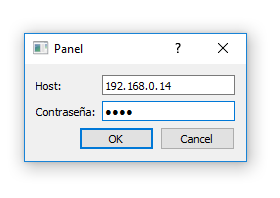
\includegraphics[scale=0.8]{imagenes/login.png}
	\caption{Captura de pantalla de la ventana de login.}
	\label{fig:login}
\end{figure}

\paragraph{Client}
Client es la clase que implementa la interacción en si a nivel mensajes de protocolo. Es decir, es la clase que sabe qué mensajes emitir y que hacer ante las respuestas.

Cuando se inicia una interacción del tipo \enquote{get}, simplemente inicia una conexión (utilizando un objeto de tipo Connection), y realiza dos interacciones en la misma conexión: una para traer el contenido del cartel y otra para traer la configuración de WiFi.

Por otro lado, cuando se inicia una interacción del tipo \enquote{set}, debe primero determinar cuales partes del módelo del cartel han cambiado y deben, por ende, ser actualizadas. Para eso usa unos métodos de SignModel que permiten cuales datos han sido cambiados por el usuario. Estos son: \code{isPasswordDirty()}, \code{isTextDirty()} y \code{isWifiConfigDirty()}.

A lo largo de una interacción, el objeto de tipo Client va cambiando de estados. Internamente tiene un enumerativo con los siguientes valores:
\begin{description}
	\item[Disconnected:] Client está listo para iniciar una interacción.
	\item[Connecting:] Se envió una solicitud de conexión y se está esperando una respuesta.
	\item[Connected:] Se recibió una respuesta a la solicitud de conexión y hay una conexión establecida.
	\item[RequestSent:] Se envió un pedido (ver sección \ref{sec:protocolo}) y se espera una respuesta.
	\item[ResponseReceived:] Se recibió una respuesta y se está procesándola.
\end{description}

Los estados Connected y ResponseReceived existen más bien por completitud, ya que el tiempo en que se permanece en esos estados no es perceptible.

También se define en esta clase un enumerativo \code{ClientError}, que representan los distintos errores en los que puede finalizar una interacción. Tiene los siguientes valores:
\begin{description}
	\item[Ok:] La interacción fue exitosa.
	\item[CertificateMissing:] No se pudo cargar el certificado TLS.
	\item[Timeout:] Se excedió el tiempo de espera a una respuesta.
	\item[WrongResponse:] Se recibió una respuesta incorrecta por parte del servidor. Esto puede suceder si hay un error en la implementación del protocolo, o si a lo que se conectó no es un cartel, sino algun otro servicio sobre TLS, como un servidor web con HTTPS.
	\item[IncompleteWrite:] No se pudo mandar un mensaje entero. Se debe a un problema externo de red.
	\item[ConnectionRefused:] El host remoto rechazó la conexión. Muy posiblemente no sea un cartel.
	\item[RemoteHostClosed:] El host remoto cerró inesperadamente la conexión. Esto puede pasar si alguna fase de la interacción tardo demasiado (por congestión de la red, por ejemplo), haciendo que el cartel cierre la conexión.
	\item[HostNotFound:] No se pudo resolver la dirección IP del nombre de host dado.
	\item[NetworkError:] Error de red genérico.
	\item[SslHandshakeFailed:] Falló el establecimiento de una conexión TLS. Esto puede darse por certificados y claves que no coinciden, corrupción de ellos o un error en la implementación de TLS del ESP8266EX.
	\item[SslInternalError:] Error interno de OpenSSL (librería que maneja las conexiones TLS).
	\item[SslInvalidData:] El certificado público cargado no es válido.
	\item[Unknown:] Error desconocido genérico.
	\item[ServerMalformedPacket:] Se recibió un paquete no conforme a lo descrito por la especificación del protocolo.
	\item[ServerBadPassword:] Se trató de iniciar una interacción con una contraseña incorrecta.
	\item[ServerBadProtocolVersion:] El cartel tiene una versión del protocolo más nueva que la de la aplicación de PC.
\end{description}
\paragraph{Connection}
Esta clase es más pequeña que las anteriores. Provee una interfaz simple para iniciar una conexión TLS y mandar mensajes. Tiene los siguientes métodos bloqueantes:
\begin{description}
	\item[\code{bool connect(const QString hostname)}:] Inicia una conexión TLS al host con nombre dado por \code{hostname}. Retorna falso si hubo error o timeout.
	\item[\code{bool disconnect()}:] Cierra la conexión. Es idempotente: si no existía previamente una conexión abierta, no realiza ninguna acción.
	\item[\code{bool send(const Message \&msg)}:] Envia el mensaje \code{msg}. Retorna falso si hay error o timeout.
	\item[\code{bool receive(Message \&msg)}:] Recibe un mensaje y lo almacena en \code{msg}. Retorna falso si hay error o timeout.
	\item[\code{QAbstractSocket::SocketError lastError()}:] Retorna un enumerativo con el último error de red. Este enumerativo es propio de Qt y luego se mapea a un valor del enumerativo \code{Client::ClientError}.
\end{description}

Todos estos métodos tienen un tiempo de expiración o \emph{timeout} definido por la constante estática \code{Connection::TIMEOUT\_MS}

